%%%%%%%%% BODY TEXT
\section{Introduction}
\label{sec:intro}
3D computer vision has been attracting a wide range of interest from academia and industry since it shows great potential in many fast-developing AI-related applications such as robotics, autonomous driving, augmented reality, \etc ~As a basic representation of 3D data, point clouds can be easily captured by 3D sensors~\cite{endres20133,jaboyedoff2012use}, incorporating the rich context of real-world surroundings.

Unlike well-structured 2D images, point cloud data has inherent properties of \emph{irregularity} and \emph{sparsity}, posing enormous challenges for high-level vision tasks such as point cloud classification~\cite{qi2017pointnet,wang2019dynamic,qiu2021geometric}, segmentation~\cite{qi2017pointnet++,qiu2021dense,hu2020randla}, and object detection~\cite{qi2019deep,qi2020imvotenet,qiu2021investigating}. For instance, Uy~\etal~\cite{uy2019revisiting} fail to classify the real-world point clouds while they apply a pre-trained model of synthetic data; and recent 3D segmentation and detection networks~\cite{hu2020randla,qiu2021semantic,Park_2021_ICCV} achieve \emph{worse} results on the distant/smaller objects (\eg, bicycles, traffic-signs) than the closer/larger objects (\eg, vehicles, buildings). If we mitigate point cloud data's \emph{irregularity} and \emph{sparsity}, further improvements in visual analysis can be obtained (as verified in~\cite{ye2021meta}). Thus, point cloud upsampling deserves a deeper investigation.

\begin{figure*}
\begin{center}
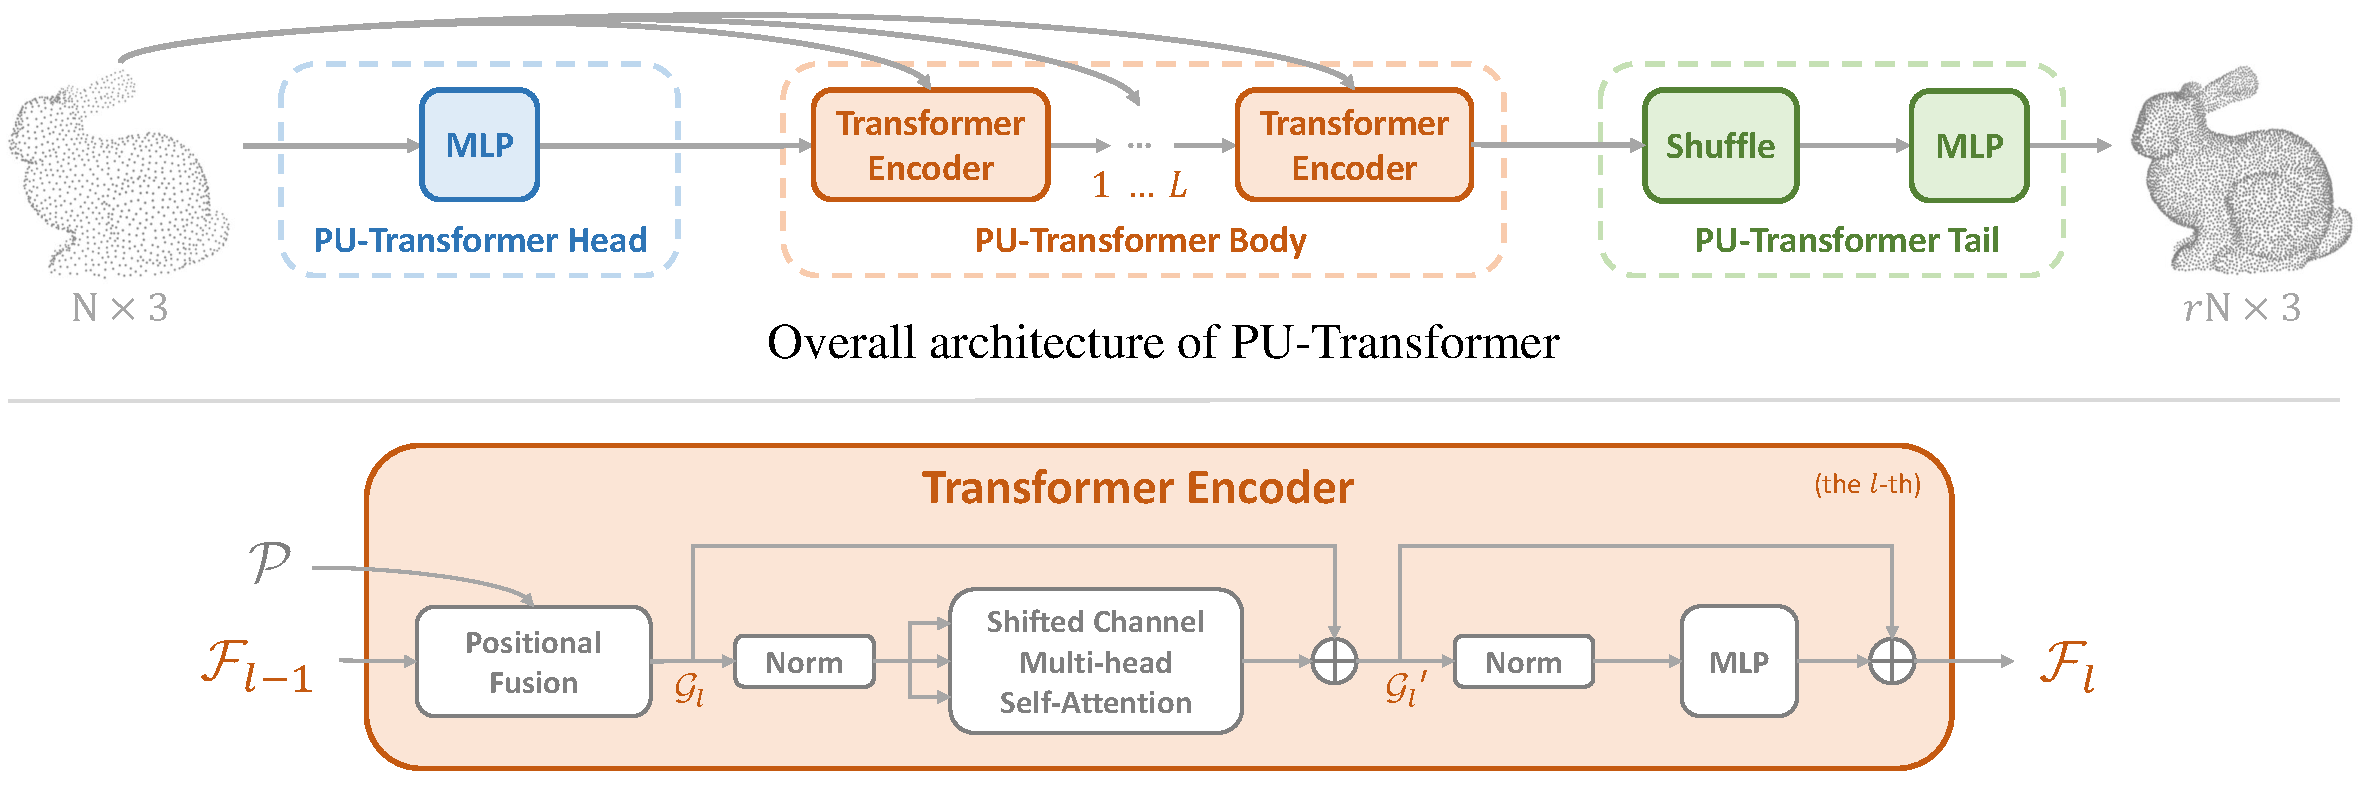
\includegraphics[width=0.9\textwidth]{images/net.pdf}
\end{center}

\captionsetup{font=small}
\caption{The details of PU-Transformer. The upper chart shows the overall architecture of the PU-Transformer model containing three main parts: the PU-Transformer head (Sec.~\ref{sec:head}), body (Sec.~\ref{sec:pu_body}), and tail (Sec.~\ref{sec:tail}). The PU-Transformer body includes a cascaded set of Transformer Encoders (\eg, $L$ in total), serving as the core component of the whole model. Particularly, the detailed structure of each Transformer Encoder is shown in the lower chart, where all annotations are consistent with Line 3-5 in Alg.~\ref{alg:put}.}
\label{fig:net}

\end{figure*}

As a basic 3D low-level vision task, point cloud upsampling aims to generate dense point clouds from sparse input, where the generated data should recover the fine-grained structures at a higher resolution. Moreover, the upsampled points are expected to lie on the underlying surfaces in a uniform distribution, benefiting downstream tasks for both 3D visual analysis~\cite{liu2019relation,qiu2021pnp} and graphic modeling~\cite{mitra2003estimating,mitra2004registration}. Following the success of Convolution Neural Networks (CNNs) in image super-resolution~\cite{dong2015image,kim2016accurate,anwar2020deep} and Multi-Layer-Perceptrons (MLPs) in point cloud analysis~\cite{qi2017pointnet,qi2017pointnet++}, previous methods tended to upsample point clouds via complex network designs (\eg, Graph Convolutional Network~\cite{qian2021pu}, Generative Adversarial Network~\cite{li2019pu}) and dedicated upsampling strategies (\eg, progressive training~\cite{yifan2019patch}, coarse-to-fine reconstruction~\cite{liu2020spu}, disentangled refinement~\cite{li2021point}). As far as we are concerned, these methods share a key to point cloud upsampling: learning the representative features of given points to estimate the distribution of new points. Considering that regular MLPs have limited-expression and generalization capability, we need a more powerful tool to extract fine-grained point feature representations for high-fidelity upsampling. To this end, we introduce a succinct transformer model, PU-Transformer, to effectively upsample point clouds following a simple pipeline as illustrated in Fig.~\ref{fig:net}. The main reasons for adopting transformers to point cloud upsampling are as follows:

\emph{Plausibility in theory.} As the core operation of transformers, self-attention~\cite{vaswani2017attention} is a set operator~\cite{zhao2021point} calculating long-range dependencies between elements regardless of data order. On this front, self-attention can easily estimate the point-wise dependencies without any concern for the inherent \emph{unorderedness}. However, to comprehensively represent point cloud features, channel-wise information is also shown to be a crucial factor in attention mechanisms~\cite{qiu2021geometric,qiu2021investigating}. Moreover, such channel-wise information enables an efficient upsampling via a simple periodic shuffling~\cite{shi2016real} operated on the channels of point features, saving complex designs~\cite{liu2020spu,li2019pu,li2021point,yifan2019patch} for upsampling strategy. Given these facts, we propose a Shifted Channel Multi-head Self-Attention (SC-MSA) block, which strengthens the point-wise relations in a multi-head form and enhances the channel-wise connections by introducing the overlapping channels between consecutive heads.

\emph{Feasibility in practice.} Since the transformer model was originally invented for natural language processing; its usage has been widely recognized in high-level visual applications for 2D images~\cite{carion2020end,dosovitskiy2020image,liu2021swin}. More recently, Chen~\etal~\cite{chen2021pre} introduced a pre-trained transformer model achieving excellent performance on image super-resolution and denoising. Inspired by the transformer's effectiveness for image-related low-level vision tasks, we attempt to create a transformer-based model for point cloud upsampling. Given the mentioned differences between 2D images and 3D point clouds, we introduce the Positional Fusion block as a replacement for positional encoding in conventional transformers: on the one hand, local information is aggregated from both the \emph{geometric} and \emph{feature} context of the points, implying their 3D positional relations; on the other hand, such \emph{local} information can serve as complementary to subsequent self-attention operations, where the point-wise dependencies are calculated from a \emph{global} perspective. 

\emph{Adaptability in various applications.} Transformer-based models are considered as a luxury tool in computer vision due to the huge consumption of data, hardware, and computational resources. However, our PU-Transformer can be easily trained with a \emph{single} GPU in a few hours, retaining a similar model complexity to regular CNN-based point cloud upsampling networks~\cite{yu2018pu,yifan2019patch,li2021point}. Moreover, following a patch-based pipeline~\cite{yifan2019patch}, the trained PU-Transformer model can effectively and flexibly upsample different types of point cloud data, including but not limited to regular object instances or large-scale LiDAR scenes (as shown in Fig.~\ref{fig:vis},~\ref{fig:vis_scan} and~\ref{fig:scan}). Starting with the upsampling task in low-level vision, we expect our approach to transformers will be affordable in terms of resource consumption for more point cloud applications. Our main contributions are:
\begin{itemize}
\item
To the best of our knowledge, we are the first to introduce a transformer-based model\footnote{The project page is: \url{https://github.com/ShiQiu0419/PU-Transformer}.} for point cloud upsampling.

\item We quantitatively validate the effectiveness of the PU-Transformer by significantly outperforming the results of state-of-the-art point cloud upsampling networks on two benchmarks using three metrics.

\item The upsampled visualizations demonstrate the superiority of PU-Transformer for diverse point clouds.
\end{itemize}